\documentclass[journal,10pt]{IEEEtran}
\usepackage[T1]{fontenc}
\usepackage[utf8]{inputenc}
\usepackage{cite}
\usepackage{amsmath,amssymb}
\usepackage{graphicx}
\usepackage{booktabs,array,tabularx}
\usepackage{xurl}
\usepackage[hidelinks]{hyperref}
\usepackage{microtype}
\usepackage{balance}
\usepackage{enumitem}
\usepackage{placeins}
\setlist[itemize]{leftmargin=*,nosep}
\setlist[enumerate]{leftmargin=*,nosep}
\newcolumntype{Y}{>{\raggedright\arraybackslash}X}
\hyphenation{scatter-ometer repro-duc-ibility pre-dictor meta-data}
\hypersetup{pdftitle={Outcome-Blind Readiness Assessment of a 128-File Coastal ASCAT Benchmark},pdfauthor={Yichen Zhu, Mutong Li, Yongzhi Li, Guanchao Tong},pdfsubject={Manuscript prepared for IEEE Transactions on Geoscience and Remote Sensing}}

\begin{document}
\title{Outcome-Blind Readiness Assessment of a 128-File Coastal ASCAT Benchmark}
\author{Yichen~Zhu, Mutong~Li, Yongzhi~Li, and Guanchao~Tong%
\thanks{\textit{Mutong Li and Yongzhi Li share second authorship.} (Corresponding author: Guanchao Tong.)}%
\thanks{Yichen Zhu, Mutong Li, and Yongzhi Li are with Wenzhou-Kean University, Wenzhou 325060, China.}%
\thanks{Guanchao Tong is with the College of Science, Mathematics and Technology, Wenzhou-Kean University, Wenzhou 325060, China (e-mail: \mbox{\href{mailto:tguancha@kean.edu}{tguancha@kean.edu}}).}}
\maketitle
\begin{abstract}
Public access to a satellite archive does not guarantee enough eligible observations in a selected benchmark. We assess a fixed benchmark of coastal ultra-high-resolution Advanced Scatterometer observations from the National Oceanic and Atmospheric Administration, using a workflow that recorded no access to reference buoy winds. The design comprised 128 satellite files and 12 stations, with eight evaluation stations assessed over five consecutive 28-day blocks. Readiness required at least 400 unique station--observation opportunities overall and at least eight in every station--block cell. After processing 96 primary files and four prespecified rounds of eight additional files, the design yielded 150 opportunities. The minimum cell count was zero, and only three of 40 cells reached eight. Wind-performance evaluation therefore did not proceed. The original repository record reports zero reads of National Data Buoy Center wind outcomes; a later deterministic replay found no outcome paths or fields and reproduced the capacity decision, terminal counts, transfer accounting, and predictor-file integrity. In the 1,024 evaluation station--file records, 628 ended without a spatial match under the specified rule. The five-stage acquisition sequence used 9.418 decimal GB. These results describe the selected files and processing rules, rather than archive-wide coverage or physical causes of missing observations. Because the audit was formulated after the capacity failure, its findings are exploratory. The study provides an inspectable readiness procedure and a negative case in which a benchmark was stopped at its predictor-only stage. Passing the subsequent integrity audit did not change the failed readiness decision.
\end{abstract}

\begin{IEEEkeywords}
Advanced Scatterometer (ASCAT), benchmark design, coastal winds, data provenance, reproducibility.
\end{IEEEkeywords}
\section{Introduction}
\IEEEPARstart{C}{oastal} wind benchmarks using Advanced Scatterometer (ASCAT) observations can fail before wind evaluation if spatial matching, quality rules, and deduplication leave too few eligible station--observation pairs. Reproducible evaluation requires this design-specific support to be documented \cite{kedron2022}. Validation of NOAA's near-real-time coastal processor establishes product performance under the conditions studied \cite{soisuvarn2023}, but does not establish support for a particular station--time design. We use \emph{benchmark readiness} for sufficient predictor support under a declared evaluation rule.

Checking readiness before authorized reference-outcome access limits outcome-dependent design changes. Replacing sparse stations or relaxing inclusion rules after examining reference winds raises leakage concerns \cite{kapoor2023}, motivating an explicit separation between prespecified decisions and post hoc repairs \cite{nosek2018}.

Our case began as a wind-performance study with eight evaluation stations, four development stations, and five 28-day blocks. Its fixed sequence of 96 primary files and four eight-file alternate rounds had to provide at least 400 evaluation opportunities overall and eight per station--block cell. Only the next complete round could be activated; individual file replacement, station substitution, and threshold relaxation were prohibited. Both requirements remained unmet after all 128 files were processed, stopping performance evaluation.

The subsequent audit reconstructed that decision from predictor-side records. Capacity and replay integrity yield distinct verdicts: a consistent replay can reproduce a capacity failure without reversing it. Because the audit was formulated after the failure was known, it remains exploratory.

The methodological focus is the integration of unique station--observation counting, a conjunctive total-and-cell gate, whole-round acquisition, final processing states, and a separate replay-integrity verdict. The reported case contains 150 opportunities; its decompositions locate the shortfall across stations, file strata, and acquisition stages. This single-design evidence establishes neither archive-wide scarcity, an optimal selection method, nor wind-retrieval performance. Independent reconstruction still requires the original implementation and inputs.

\section{Related Work}
\subsection{Coastal ASCAT observations}
ASCAT's separated observing swaths prevent nominal coverage from guaranteeing observations at a particular coastal station \cite{eumetsat2022,wmo2026}. Coastal retrievals also depend on resolution, land contamination, and quality-control choices. Verhoef \emph{et al.}\ studied high-resolution coastal winds \cite{verhoef2012}, and Lindsley \emph{et al.}\ validated high-resolution retrievals \cite{lindsley2016}. More recently, Soisuvarn \emph{et al.}\ described NOAA's coastal processor, including land correction, quality control, and validation \cite{soisuvarn2023}. These studies establish the product context. The present audit instead examines whether a fixed selection supplies the predictor opportunities required by its evaluation plan; it recorded no reference-wind access or model scores.

\subsection{Analysis-ready data and fitness for purpose}
Analysis-ready processing \cite{dwyer2018} and quality-assurance guidance \cite{qa4eo2010} address consistent inputs and fitness-for-purpose evidence, while dataset documentation records composition and limitations \cite{gebru2021}. The requirement examined here is local support after the benchmark's spatial, candidate, and deduplication rules: consistently processed products may still leave planned station--time comparisons underpopulated. The counting and stopping rules make that design-specific requirement explicit.

\subsection{Prespecification and workflow provenance}
Prespecification separates planned decisions from post hoc repair \cite{nosek2018}; Registered Reports add prospective peer review \cite{chambers2015}. Here, only a repository-local freeze preceded recorded wind-outcome access. The later audit was defined after the capacity failure and remains exploratory.

PROV-DM models entities, activities, agents, and derivations \cite{prov2013}; RO-Crate packages research objects with metadata \cite{rocrate2022}. The 2024 Workflow Run RO-Crate framework extends this approach to workflow-execution provenance \cite{leo2024}, while BagIt addresses packaging and checksum-based fixity \cite{bagit2018}. The examined implementation uses hashes, typed records, and run receipts for related purposes, without claiming standards conformance.

The 2025 STAC standard describes spatiotemporal assets and their links \cite{stac2025}, and cloud-native repositories support scalable scientific-array access \cite{abernathey2021}. These developments can support discovery and traceability, but a readiness assessment still requires application-specific counting units, thresholds, repair rules, and decision semantics.

The original literature map covered 15 sources on 4 November 2026, with two interoperability references added on 12 November. This targeted search cannot establish exhaustive novelty. We therefore present an integration of existing principles in a documented coastal ASCAT case.

\section{Study Design and Evidence Boundary}
\label{sec:identity}
\subsection{The source performance protocol}
The source workflow, version 4.1, was intended to evaluate wind performance in stages. Its initial stage, B0, used predictor information only. It fixed station roles, satellite files, time blocks, predictor extracts, opportunity counts, processing states, transfer records, and later evaluation rules before any recorded request for National Data Buoy Center (NDBC) wind outcomes. A capacity gate, denoted G0-v4.1, controlled entry to B1. Only a pass could authorize access to outcomes at the four development stations. Outcomes at the eight evaluation stations would remain sealed until a later evaluation stage.

The gate required at least 400 unique evaluation opportunities and at least eight opportunities in every evaluation station--block cell. If the 96 primary files did not meet both requirements, the next complete eight-file alternate round could be activated. Four rounds were permitted. The protocol prohibited selecting individual files from a round, substituting stations, relaxing thresholds, or inspecting reference winds to decide how to repair the design.

All four rounds were exhausted without meeting the rule. The workflow recorded G0-v4.1 as failed and stopped with \texttt{FAIL\_EXHAUSTED}; B1 remained closed. Consequently, no wind model fitting, performance comparison, calibration analysis, or evaluation score was produced. The planned performance hypotheses remained untested.

\subsection{The subsequent integrity audit}
Version 5 was a separate audit defined after the capacity failure. It inherited the selected files, station roles, blocks, thresholds, processing states, and opportunity keys. Its purpose was to reconstruct the recorded decision without changing those inputs or reading wind outcomes.

The audit gate, G0-v5, tests consistency of that reconstruction. It compares input hashes, identifiers, counts, keys, processing-state distributions, transfer totals, raw-file disposition, predictor-file properties, gate states, and outcome-read counters with the preserved record. A pass means that the replay agrees with the source evidence; it does not mean that the benchmark has become ready for performance evaluation. Figure~\ref{fig:workflow} summarizes these two decisions.

\begin{figure*}[!t]
\centering
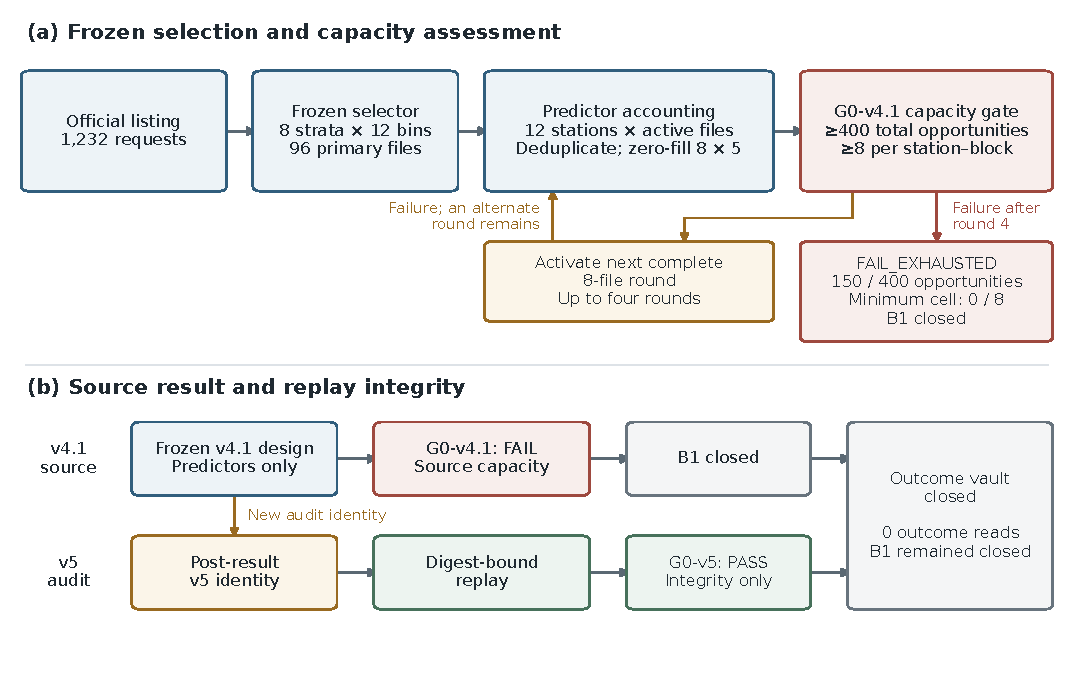
\includegraphics[width=\textwidth]{figures/figure1.pdf}
\caption{Readiness assessment and subsequent replay. The source workflow selects and processes files without opening buoy-wind outcomes, counts unique station--observation opportunities, and activates complete alternate rounds when needed. Failure after the final round stops performance evaluation. The later integrity audit checks the preserved failure record; its pass does not reverse the source decision.}
\label{fig:workflow}
\end{figure*}

The evidence boundary is the original repository record. Its counters report zero NDBC outcome reads, and the replay found no outcome paths or fields among its allowed inputs. This is an internal consistency claim, not a demonstration of external execution isolation. Because the audit was formulated after the capacity result was known, all findings in this paper remain exploratory.

\section{Materials and Methods}
\subsection{Public sources and study period}
The source study used official, account-free NOAA services. Satellite files were selected from \url{https://manati.star.nesdis.noaa.gov/UHR_COASTAL/}, without redirects or credentials. A listing inventory of 1,232 requests was collected on 4 November 2026 between 06:39:16 and 07:22:46 UTC and bound to the protocol by cryptographic digests. Listing metadata defined the candidate universe; they did not establish each file's original dissemination time, continued availability, or processor version.

The study interval was 17 June 2026, 00:00 UTC, through 4 November 2026, 00:00 UTC, with the final endpoint excluded. Five consecutive 28-day blocks began on 17 June, 15 July, 12 August, 9 September, and 7 October. The eight evaluation stations were 41047, 42001, 42035, 42036, 42056, 44008, 44014, and 44020. The four development stations were 41008, 42002, 42039, and 44027. Figure~\ref{fig:stations} places the reported station coordinates in their geographic context; the roles and original selection labels are listed in Supplementary Table~S1.

Station selection used official static metadata and time coordinates. Within each region, eligible stations were divided into four latitude-rank bins, and a stable salted hash selected one evaluation station per bin. The remaining candidates were repartitioned into two bins per region; a different salt selected disjoint development stations. This separation was introduced in the version-4-to-4.1 protocol repair before recorded wind-outcome access. No wind speed, wind direction, or outcome-side ancillary variable was used in the selection.

\begin{figure*}[!t]
\centering
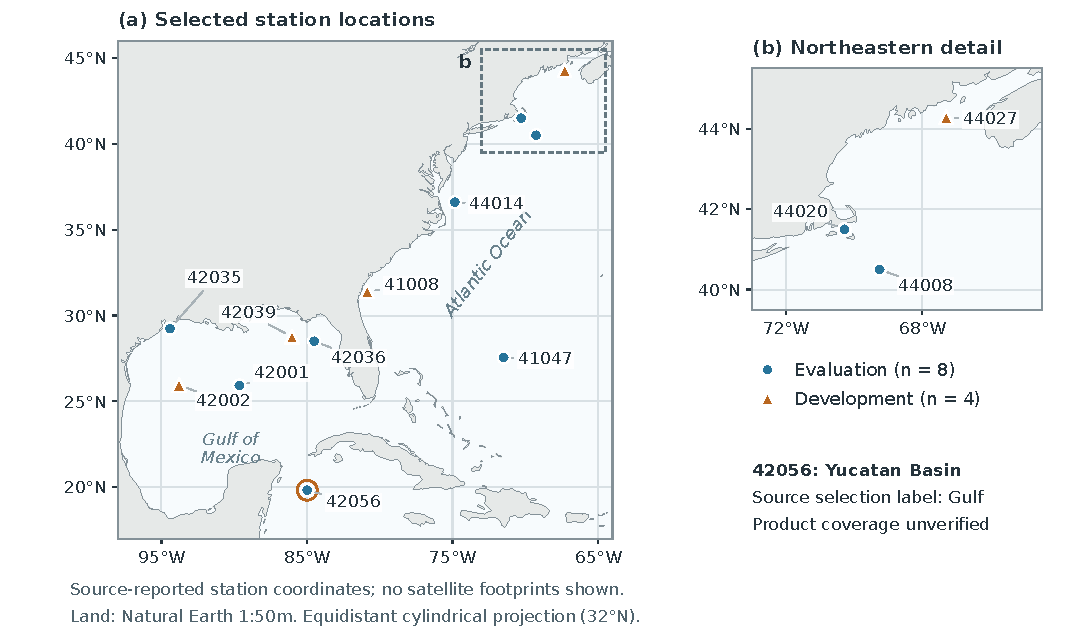
\includegraphics[width=\textwidth]{figures/station_map.pdf}
\caption{Reported station locations and study roles. Coordinates are transcribed from the source study's period-median deployment record. The northeastern inset separates nearby stations. Land outlines use Natural Earth at 1:50 million scale \cite{naturalearthland}. This is a geographic context map, not a satellite-coverage map. Station 42056 retains the original Gulf selection label; its association with the selected product footprints remains unverified.}
\label{fig:stations}
\end{figure*}

\subsection{File selection and alternate rounds}
Eight file strata crossed the Atlantic and Gulf product sectors (\texttt{ec}/\texttt{gc}), MetOp-B and MetOp-C, and ascending and descending passes. Each stratum was divided into 12 equal time bins. One salted-hash minimum per stratum and time bin supplied the 96 primary files.

A logical satellite observation was identified by platform/pass prefix, sensing time, orbit, and sector. Only base variants were eligible. Revisions were resolved by highest revision and then lexical stem order; the filename was not treated as evidence of processor version. A separate salted ordering of nonprimary observations supplied four alternate rounds, each containing one file from every stratum. Thus the entire selectable set was fixed at 128 files before opportunity counts determined how many rounds to activate.

All active extracts had to reach a final processing state before a capacity decision. Counts could trigger the next whole round, but could not change its order or select individual files within it. Development-station counts were report-only and could neither activate a round nor satisfy the evaluation gate. Complete rounds maintained balanced increments across the eight strata. The policy was a control on adaptive file choice, not an attempt to maximize yield per downloaded byte.

\begin{table*}[!t]
\caption{Fixed benchmark design and capacity rule}
\label{tab:design}
\centering\small
\begin{tabularx}{\textwidth}{@{}p{0.19\textwidth}Y Y@{}}
\toprule
Element & Specification & Meaning for this audit \\
\midrule
Study population & 128 selectable files; 8 evaluation and 4 development stations & Only evaluation opportunities contribute to the capacity gate. \\
File strata & 2 sectors $\times$ 2 platforms $\times$ 2 pass directions & 96 primary files from 12 time bins per stratum. \\
Repair policy & Four ordered rounds of 8 alternate files & Whole rounds only; no file substitution or reordering. \\
Period & 17 June--4 November 2026, UTC; final endpoint excluded & Five consecutive 28-day blocks; 40 evaluation cells. \\
Counting unit & Unique station--logical-observation pair & A $5\times5$ neighborhood contributes at most one opportunity. \\
Spatial/candidate rule & Center within 12.5 km; at least 2 valid ambiguity candidates & Passing denotes protocol eligibility, not verified wind accuracy. \\
Capacity rule & At least 400 total and 8 per station--block cell & Both conditions must pass before outcomes can be opened. \\
Acquisition limits & 10,000,000,000 new science bytes; at most 2 transient raw files & 128 selected files are a bounded design, not an archive census. \\
Specification status & Repository-local freeze before recorded outcome access & No public preregistration; the later audit is exploratory. \\
\bottomrule
\end{tabularx}
\end{table*}

\subsection{Opportunity definition and quality rules}
An opportunity was one unique pair of station identifier and logical-observation key. Deterministic nearest-center selection had to locate a protocol-valid retrieval coordinate within 12.5 km of the station. Its center-pixel time had to fall within the study interval and a specified block, and a verified predictor neighborhood had to be available. Each extract contained a same-file, same-pass $5\times5$ neighborhood; out-of-bounds cells were invalid. The 25 pixels did not create additional opportunities.

Each retrieval cell could contain up to four wind-ambiguity candidates, of which at least two had to be valid. Invalid coordinates, land, ice, numerical-weather-prediction ice, missing pixel time, candidate-shape mismatch, an out-of-range selected index, and unresolved direction semantics were grounds for rejection. NOAA quality-control, rain, and anomaly-filter flags were retained as descriptors rather than used to exclude cases. Their presence therefore did not directly reduce the opportunity count. Conversely, the processing label \texttt{extract\_valid} indicates compliance with these predictor rules, not an assessment of retrieval accuracy.

If several records represented the same station--observation pair, their deterministic order was distance, absolute time difference from file sensing time, file SHA-256 digest, center row, and center column. The audit materialized all 40 evaluation station--block cells, including zeros. The 30-minute buoy-collocation tolerance specified for the later performance study was not used in this predictor-only count.

\subsection{Capacity gate and stopping condition}
Let $N_{s,b}$ denote the number of distinct opportunities at evaluation station $s$ in block $b$, and let $N_{\mathrm{eval}}$ be their total. With eight evaluation stations $\mathcal{S}$ and five blocks $\mathcal{B}$, the gate passes only when
\begin{equation}
N_{\mathrm{eval}}\geq400
\quad\text{and}\quad
\min_{s\in\mathcal{S},\,b\in\mathcal{B}}N_{s,b}\geq8.
\label{eq:gate}
\end{equation}
The rule is evaluated after the primary files and after every complete alternate round. An intermediate failure activates the next round. Failure after round 4 stops the workflow with \texttt{FAIL\_EXHAUSTED} and leaves B1 unauthorized.

The planned downstream analysis required at least 320 cases overall and six per cell. The predictor thresholds of 400 and eight therefore allowed 20\% aggregate and 25\% cell-level attrition before those minima would be violated. These margins explain the relationship between the two configured gates. They were not derived from a statistical power or precision calculation.

\subsection{Processing states and transfer accounting}
Each of the $128\times12=1{,}536$ station--file combinations required one final state: a valid extract, fewer than two valid candidates, no spatial overlap under the specified rule, or invalid time. The corresponding stored labels were \texttt{extract\_valid}, \texttt{fewer\_than\_two\_valid\_candidates}, \texttt{no\_overlap}, and \texttt{time\_invalid}. These labels describe the workflow's disposition of a record; they do not identify a physical cause.

Final-key accounting also required one selection record and one transfer record per selected source, and one predictor-case record per evaluation opportunity. Earlier transfer attempts remained linked to their parents. Downloaded objects were distinguished from preexisting geometry evidence reused by digest. Probe bytes were counted separately, and no transient raw download could remain when the transaction closed.

The inventory and extract denominators describe different objects. The 1,232-request listing inventory includes 560 date-prefix requests within the study interval. Of those 560, 141 carried the combined label \texttt{public\_endpoint\_empty\_or\_not\_backfilled}. This label does not distinguish absence of an observation from the state of the public listing or backfill. The station--file tables, in contrast, include every selected file paired with every station in the relevant role; their denominators are not estimates of expected physical overpasses.

\subsection{Deterministic replay and integrity checks}
The replay read eight declared inputs: the source opportunity report, transaction receipt, selection ledger, transfer ledger, station-extract manifest, station-role manifest, evaluation-case Parquet, and a tree of 128 per-file predictor receipts. It also bound six evaluator artifacts: the inherited opportunity, terminal-state, and pre-outcome-freeze contracts, together with the later audit commitment, claim map, and replay specification. File or tree digests were checked before parsing.

The replay rejected network locations, path traversal, undeclared inputs, outcome-like paths, and prohibited outcome fields. From the allowed inputs it recomputed file membership, station roles, block identities, opportunity keys, the zero-filled count matrix, stage contributions, processing-state distributions, final-key closure, transfer-attempt parent chains, byte totals, raw-file disposition, and Parquet properties. It also checked the explicit outcome-read counters and the different meanings of the source and audit gates. Thirteen integrity checks had to pass without disagreement.

The three final outputs had to be absent before execution. A lock protected the transaction; the comparison ledger and narrative were committed before the final JSON receipt. Bound inputs were checked again before the receipt was written, and output bytes were checked afterward. This procedure checks repository-local consistency and detects incomplete output states. It does not establish power-loss atomicity or isolation from an unrelated process changing files concurrently.

\subsection{Audit scope and statistical treatment}
The original record contains one eligible version-5 replay run, identified as \texttt{RUN-R1-V5-B0-FEASIBILITY-REPLAY-A1}. It was linked to both audit claims and verified by a non-owner within the same research environment. The subsequent result audit included that run and excluded none. It recorded agreement for protocol, metrics, outcome accounting, provenance, and continuity, but failed its formal independence check because the audit shared the source implementation and repository context. The resulting classification was exploratory support rather than independent confirmation.

For the descriptive acquisition profile, each alternate round's marginal yield was its additional evaluation opportunities divided by the volume of additional transferred science data in decimal GB. This ratio summarizes the realized sequence and does not compare unexecuted policies.

All reported counts enumerate the selected universe. They are not estimates obtained from a probability sample of the wider NOAA archive. We therefore report neither confidence intervals nor significance tests. Generalization to other file selections, stations, or periods requires a separately specified population and analysis design. Supplementary material lists the execution commands and artifact paths reported for the source study. Independent reproduction is outside the evidence provided here.

\section{Results}
\label{sec:results}

\subsection{The design did not meet its capacity requirements}
After the 96 primary files and all four alternate rounds had been processed, the evaluation set contained 150 unique station--observation opportunities. This was 37.5\% of the required total of 400. The smallest station--block count was zero, and only three of the 40 cells reached the requirement of eight. Both parts of the capacity rule therefore failed. The source workflow recorded \texttt{G0\_NOT\_PASSED} and \texttt{FAIL\_EXHAUSTED}, leaving the outcome-reading stage B1 unauthorized. These decisions concern support for the planned benchmark; the percentage does not measure archive completeness or wind-retrieval performance.

Table~\ref{tab:gate-results} distinguishes this capacity decision, \texttt{G0-v4.1}, from the subsequent replay-integrity decision, \texttt{G0-v5}. The replay passed because it reproduced the unsuccessful capacity check and its supporting records. It did not add observations or authorize the original performance experiment.

\begin{table*}[t]
\caption{Capacity and replay decisions. A successful replay does not change the capacity result.}
\label{tab:gate-results}
\centering
\small
\begin{tabularx}{\textwidth}{@{}p{0.14\textwidth}p{0.23\textwidth}p{0.24\textwidth}X@{}}
\toprule
Decision & Observed result & Requirement & Consequence \\
\midrule
Capacity: \texttt{G0-v4.1} &
150 opportunities; minimum cell count 0; 3 of 40 cells reach 8 &
At least 400 overall and at least 8 in every station--block cell &
Failed after all alternate rounds; B1 remained closed. \\
Replay: \texttt{G0-v5} &
62 of 62 comparisons agree; 13 of 13 integrity checks pass &
Agreement with the sealed inputs, counts, decisions, and outcome-access record &
The capacity failure was reproduced; no performance evaluation was authorized. \\
\bottomrule
\end{tabularx}
\end{table*}

Figure~\ref{fig:capacity} shows the complete matrix, including zero-count cells. Station totals ranged from zero at 42056 to 35 at 44020; station 41047 contributed one opportunity. The remaining totals were 22 at 42001, 29 at 42035, 14 at 42036, 30 at 44008, and 19 at 44014. The three qualifying cells were 42035 in Block~4 and 44008 in Block~1, each with eight opportunities, and 44020 in Block~4, with nine. Thus, the shortfall was not confined to the overall total: most of the intended station--time comparisons also lacked the required support.


\begin{figure}[!t]
\centering
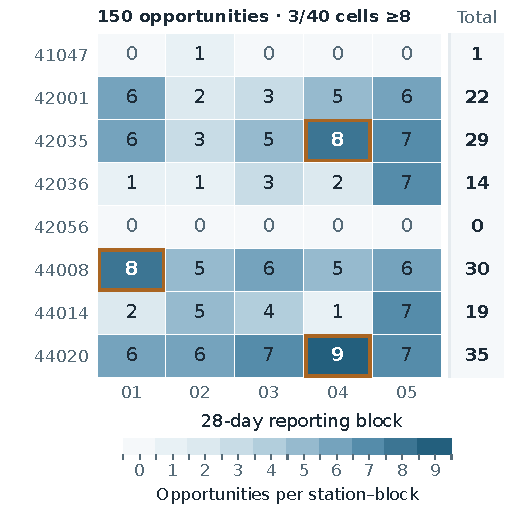
\includegraphics[width=\columnwidth]{figures/figure2.pdf}
\caption{Unique station--observation opportunities in the eight-station, five-block design. All cells, including zeros, are shown. Outlined cells reach the required eight opportunities; three of 40 do so.}
\label{fig:capacity}
\end{figure}

\subsection{Terminal states and the distribution of the shortfall}
Every one of the 1,536 station--file combinations received a final processing state. Of the 1,024 evaluation rows, 150 were valid extracts, 35 failed the two-candidate requirement, 628 had no spatial overlap, and 211 had an invalid time. The corresponding development counts were 68, 30, 271, and 143, totaling 512. Across both roles, the four counts were 218, 65, 899, and 354. Table~\ref{tab:accounting} summarizes these totals and the principal integrity checks; Fig.~\ref{fig:terminals} displays the role-specific composition.

The stored labels are \texttt{extract\_valid}, \texttt{fewer\_than\_two\_valid\_candidates}, \texttt{no\_overlap}, and \texttt{time\_invalid}. They identify the condition at which processing ended. A valid extract satisfies the predictor protocol but is not a claim of accurate wind retrieval; similarly, a failed extract does not by itself identify a physical cause.

\begin{table*}[t]
\caption{Terminal-state counts and principal record checks. Terminal counts use station--file rows, whereas the case manifest uses unique station--observation opportunities.}
\label{tab:accounting}
\centering
\small
\begin{minipage}[t]{0.48\textwidth}
\vspace{0pt}
\begin{tabularx}{\linewidth}{@{}Xrr@{}}
\toprule
Terminal state & Evaluation & Development \\
\midrule
Valid extract & 150 & 68 \\
Fewer than two valid candidates & 35 & 30 \\
No spatial overlap & 628 & 271 \\
Invalid time & 211 & 143 \\
\midrule
Total & 1,024 & 512 \\
\bottomrule
\end{tabularx}
\end{minipage}
\hfill
\begin{minipage}[t]{0.49\textwidth}
\vspace{0pt}
\begin{tabularx}{\linewidth}{@{}Xr@{}}
\toprule
Record check & Reported value \\
\midrule
Unique final keys & 1,942 \\
Retained nonfinal attempts & 253 \\
Parquet rows $\times$ ordered fields & $150\times22$ \\
Downloaded / reused source files & 125 / 3 \\
Transient raw files at closure & 0 \\
Recorded NDBC outcome reads & 0 \\
\bottomrule
\end{tabularx}
\end{minipage}
\end{table*}


\begin{figure}[!t]
\centering
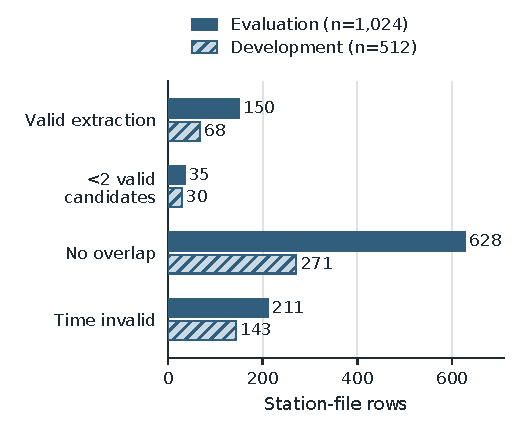
\includegraphics[width=\columnwidth]{figures/figure3.pdf}
\caption{Processing-state counts by station role. Evaluation and development denominators are 1,024 and 512 station--file records, respectively. The bars show counts, not rates; the state labels do not identify physical causes.}
\label{fig:terminals}
\end{figure}

\subsection{Opportunity gains along the prescribed acquisition sequence}
The primary set yielded 114 opportunities from 96 files and used 7,003,624,776 new science bytes. Successive complete alternate rounds added 11, 9, 11, and five opportunities, taking the cumulative totals to 125, 134, 145, and 150. Figure~\ref{fig:budget} plots the five realized stages. The additional byte costs were 610,514,454; 596,205,693; 590,329,239; and 617,772,188, respectively. Round~4 therefore had the lowest observed marginal opportunity yield. Exact cumulative values are retained in the supplementary inventory.

The complete sequence used 9,418,446,350 new science bytes, or 9.418 decimal GB. This left 581,553,650 bytes below the 10,000,000,000-byte limit, but no further alternate round was permitted. The final stop followed exhaustion of the registered file sequence, not depletion of every remaining byte. The five plotted points describe that sequence only; they do not establish an optimal file-selection policy or a budget frontier.


\begin{figure}[!t]
\centering
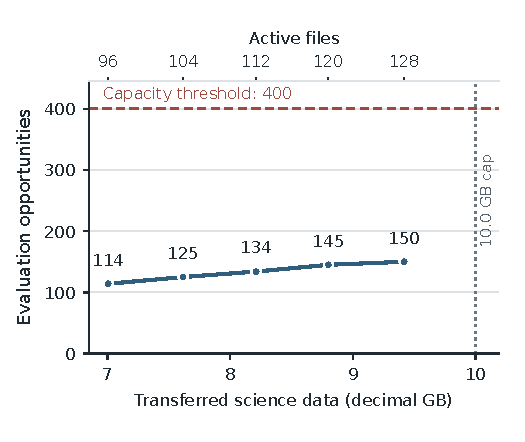
\includegraphics[width=\columnwidth]{figures/figure4.pdf}
\caption{Cumulative evaluation opportunities and acquisition cost after the primary set and each complete alternate round. Cost is in decimal GB and includes probe bytes. The points describe the executed sequence; the dashed line is the required total of 400 opportunities.}
\label{fig:budget}
\end{figure}

\subsection{Diagnostics by file stratum, station, and time block}
The further decompositions in Fig.~\ref{fig:diagnostics} use all 1,024 evaluation rows. No overlap was the largest category in each sector--platform--pass stratum, ranging from 72 of 128 rows (56.25\%) in both Atlantic MetOp-B strata to 84 of 128 (65.63\%) in the Atlantic MetOp-C descending and Gulf MetOp-B ascending strata. Atlantic-sector files contributed 89 valid opportunities and Gulf-sector files contributed 61.

The station breakdown was more uneven. All 128 rows at 42056 ended in no overlap, as did 112 of 128 at 41047. Invalid times were most frequent at 42036, with 50 of 128 rows. All rows in the block breakdown were grouped by source-file sensing time, because failed records lack a valid center-pixel block. Its denominators were consequently 184, 224, 176, 224, and 216, rather than equal-sized groups. These displays locate the recorded losses within the selected design; they do not separate station geography, orbit geometry, retrieval behavior, or archive state as explanations.


\begin{figure*}[!t]
\centering
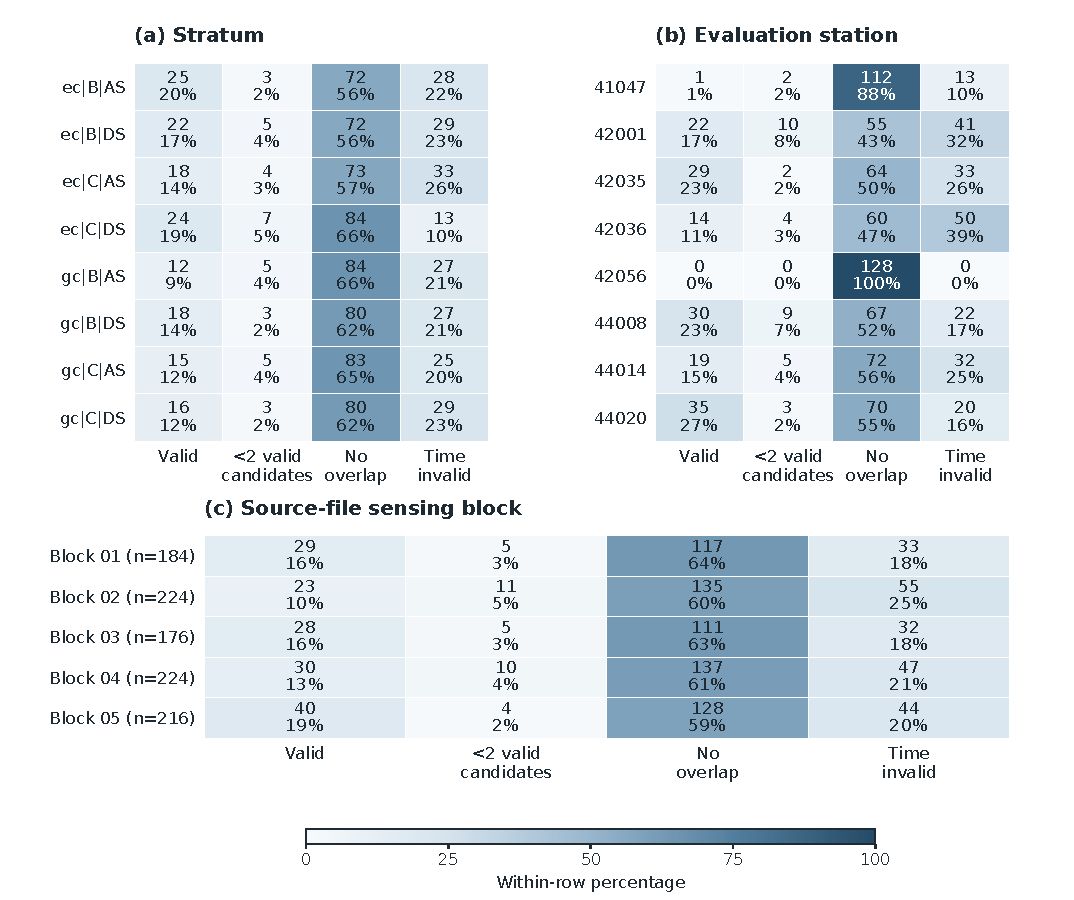
\includegraphics[width=\textwidth]{figures/figure5.pdf}
\caption{Evaluation processing states by (a) sector--platform--pass stratum, (b) station, and (c) source-file sensing block. In (a), ec/gc denote the Atlantic/Gulf product sectors, B/C denote MetOp-B/MetOp-C, and AS/DS denote ascending/descending passes. Cells show counts and within-row percentages. Each row in (a) and (b) has 128 records; the block denominators in (c) differ. All records in panel (c) are grouped by file sensing time, because failed records lack a valid center-pixel time. These are descriptive processing categories, not causal diagnoses.}
\label{fig:diagnostics}
\end{figure*}

\subsection{Closure, transfer accounting, and replay agreement}
The final record contained 128 selected-source keys, 128 source-transfer keys, 1,536 station-extract keys, and 150 predictor-case keys: 1,942 in total. No expected final key was missing or duplicated. A further 253 nonfinal attempts remained in the lineage with valid parent chains.

Of the 128 source files, 125 were newly downloaded and three reused existing geometry evidence with matching digests. Downloaded objects accounted for 9,418,445,350 bytes. The transaction added 1,000 probe bytes, consistent with 125 eight-byte probes, to obtain the total acquisition cost above. All newly downloaded raw files were deleted after their extracts had been verified; the three reused geometry files were retained.

The evaluation Parquet contained 150 rows and 22 ordered fields. It had 150 unique case identifiers and 150 unique station--observation keys. The file digest, schema digest, \texttt{PAR1} signature, dimensions, uniqueness checks, and reopen check agreed with the recorded contract. No prohibited outcome field was present.

The replay produced 62 ledger comparisons, all with matching observed and expected values, and passed all 13 registered integrity checks. The NDBC outcome-read counter remained zero, and no outcome path or field was found among the replay inputs. Accordingly, no wind error, calibration measure, ambiguity-comparison score, or model ranking was produced.

\subsection{Provenance limitations reproduced by the audit}
\label{sec:provenance}
Two weaknesses in the source record remained despite the successful checks. First, a nested Parquet receipt points to a temporary staging location that was deleted after commit. The canonical file passes the content, schema, uniqueness, and reopening checks, but the embedded locator is no longer usable. Content integrity and locator validity are therefore different properties in this record.

Second, the transfer lineage contains 125 \texttt{probe\_ok} nodes but does not retain an individual request-and-response receipt for each successful probe. The aggregate calculation, $125\times8=1{,}000$ bytes, reconciles; it cannot independently reconstruct every response header or returned magic byte. A later release could add a locator-resolution map without changing the original receipt and retain complete per-probe receipts for new acquisitions. Neither repair has been counted here as a completed experiment.


\section{Discussion}
\label{sec:discussion}

\subsection{Availability did not provide sufficient support for this benchmark}
The study separates access to a product from support for a particular evaluation. Official files were available, 128 sources were processed, and their extracts and accounting records could be checked. Nevertheless, the selected stations and period provided only 150 of the 400 required opportunities, with most station--block cells below their local threshold. The original performance experiment could not proceed under its declared rules.

This result adds a design-specific question to the concerns addressed by analysis-ready data and quality-assurance frameworks: after the population, matching criteria, and reporting cells have been fixed, how much usable support remains for the intended comparison? Consistent processing and traceable quality information help make data usable, but do not supply the answer to that question~\cite{dwyer2018,qa4eo2010}. Nor do published coastal ASCAT validation results determine the opportunity counts for this selection~\cite{verhoef2012,lindsley2016,soisuvarn2023}. Nothing in the present counts establishes that the product is inaccurate or unsuitable for other applications.

\subsection{The stopping decision and its replay answer different questions}
The capacity gate prevented the workflow from continuing to outcomes when its support requirements were unmet. Replacing stations, extending the interval, relaxing a criterion, or choosing individual alternate files could define a useful new experiment. Those changes would not show that the original design had passed. Keeping the complete alternate rounds and stopping after their exhaustion made the distinction explicit.

The replay addressed whether that decision and its supporting arithmetic could be reconstructed. Its successful checks improve the inspectability of the recorded failure: duplicated opportunities, inflation by neighborhood pixels, missing final records, or an unexecuted prescribed alternate round do not explain the reproduced count. They do not establish the physical cause of the shortfall, independently validate the extraction software, or confer external reproducibility. Separating the capacity decision from record integrity avoids treating successful data engineering as evidence that a scientific sampling requirement has been met.

\subsection{Thresholds should follow the intended analysis}
The 400-total and eight-per-cell requirements were inherited from the original workflow. They allow losses of 20\% overall and 25\% within a cell before the downstream minima of 320 and six would be crossed. These calculations explain the relationship between the two stages; they do not justify either set of minima through statistical power or target precision.

A successor study should specify its estimand, independent analysis unit, target precision or power, relevant heterogeneity, and expected retention between predictor screening and outcome analysis. The station and file populations, local support requirements, and acquisition budget can then be set together. This would make a failed capacity check informative about a justified scientific design, rather than only about compliance with an inherited configuration. The current negative result remains useful because it identifies the support that was actually available before any reported outcome access.

\subsection{What can and cannot be learned from sensitivity calculations}
The terminal counts provide one simple upper bound. Only 35 evaluation rows failed the two-candidate rule. Even if all 35 became valid after relaxing that rule, and no other requirement changed, the total could be no greater than 185, still below 400. This is an arithmetic ceiling, not a completed one-candidate experiment. Determining the actual gain would require new selection semantics and reprocessing.

The retained material is insufficient for an analogous 15- or 20-km spatial calculation. Failed rows do not preserve the nearest center outside the 12.5-km tolerance, and the 125 downloaded raw files were deleted after extraction. A future outcome-blind study could preregister a distance-by-candidate-rule grid, reacquire the source files, and retain nearest-center distances for every terminal state. It should report the resulting counts under the new design rather than merge them into the present result.

The acquisition trace also leaves a separate optimization question open. Complete rounds maintained representation across the eight strata and prevented selection of individual files after their opportunity yields were seen. Comparing that policy with progressive activation or forecasts of orbital and buoy sampling would require a larger prespecified candidate universe, explicit objectives, and the same budget and stopping conditions. The five realized points here cannot establish which policy would be more efficient.

\subsection{Making the evidence usable beyond its original repository}
A reusable readiness record needs both the decision rule and enough information to reconstruct its inputs. The population, interval, counting unit, deduplication procedure, thresholds, alternate order, budget, outcome-access boundary, terminal definitions, digests, and stop state should travel with the result. The source manuscript reports a project-level JSON Schema for these fields; it is an implementation aid, not a community standard.

Existing infrastructures can represent complementary parts of such a release. STAC can describe the candidate assets and their spatial and temporal extents~\cite{stac2025}. RO-Crate and Workflow Run RO-Crate can link plans, software, inputs, outputs, and execution records~\cite{rocrate2022,leo2024}, while BagIt provides a payload-manifest approach to fixity~\cite{bagit2018}. Pangeo-style repositories address access to scientific arrays and scalable analysis~\cite{abernathey2021}. These are possible mappings, not standards conformance demonstrated by this implementation.

The remaining release work is concrete: resolve the stale locator, retain probe-level receipts in future acquisitions, document redistribution rights, provide a locked runtime and checksums, and deposit the permitted artifacts in a durable versioned archive. An independently implemented replay would then test reproducibility beyond the original software context, consistent with the broader reproducibility goals of remote sensing research~\cite{kedron2022}. Until those steps are completed, the evidence supports the reported design decision and its internal reconstruction.

\section{Limitations}
\label{sec:limitations}

The audit was defined after the source capacity failure was known. Inheriting the file universe, thresholds, and outcome restriction does not make it confirmatory. The earlier repository-local freeze was neither public preregistration nor prospective journal review as a Registered Report.

The sample covers one 140-day period, eight evaluation and four development stations, and 128 files selected by one policy. Results depend on the 12.5-km tolerance, candidate rules, complete alternate rounds, and configured 400/8 thresholds. They do not estimate readiness failures across the NOAA archive or validate those thresholds as sufficient for a scientific comparison.

Several mechanisms remain inseparable. The joint \texttt{public\_\allowbreak endpoint\_\allowbreak empty\_\allowbreak or\_\allowbreak not\_\allowbreak backfilled} label occurred for 141 of 560 study-interval date-prefix requests, a subset of the 1,232-request listing inventory. It does not distinguish absent observations from listing or backfill state. Terminal counts likewise combine location, file selection, tolerance, candidate eligibility, and processing rules. In particular, the 211 evaluation records labeled \texttt{time\_invalid} require underlying examples and time-decoding checks before their causes can be identified.

The source regional labels do not establish product coverage. Station 42056's Gulf selection assignment requires verification against actual file footprints; Supplementary Table~S1 retains the original label and identifies this unresolved mapping. The candidate station universe, region eligibility boundaries, hash configuration, file manifest, and extraction-field definitions are also needed to reconstruct selection and processing.

Repository counters report zero NDBC wind-outcome reads, and the replay found no outcome path or field. Wind error, ambiguity correctness, candidate containment, calibration, energy score, selection regret, and baseline ranking were not measured. The record cannot establish whether any external process or person accessed outcomes.

Section~\ref{sec:provenance} describes a deleted staging locator and absent individual probe receipts. Raw-file deletions also prevent spatial sensitivity analysis from the retained extracts alone. Digest agreement and aggregate byte reconciliation do not resolve these omissions. The transaction checks provide closure within the cooperating workflow, not power-loss atomicity or protection against a noncooperative writer.

Source verification and the claim-level audit shared the original repository and implementation. The reported non-owner review therefore does not establish independent reproduction. The original research pack is absent from the public companion release, and its code, tests, and hashes have not been independently rechecked here. The targeted literature map was not a systematic review and cannot establish methodological priority. These gaps require underlying implementation evidence and independent validation.

\section{Conclusion}
\label{sec:conclusion}

The fixed 128-file NOAA Coastal UHR ASCAT design failed its configured capacity rule: it contained 150 evaluation opportunities against 400 required, a minimum station--block count of zero, and only three of 40 cells reaching eight. Its workflow recorded zero NDBC wind-outcome reads and kept performance evaluation closed.

The reported deterministic replay reproduced the decision and supporting records while preserving two provenance defects. It illustrates why a consistent audit record and sufficient benchmark support require separate verdicts. The evidence remains specific to this selection and its thresholds; no wind-performance hypothesis was tested.

Further work should justify thresholds from the intended analysis, verify station-to-product coverage and extraction semantics, and test alternative designs prospectively. Releasing the original implementation and artifacts is necessary to make the reported workflow independently reconstructable.

\section*{Data and Code Availability}
The manuscript source, figures, transcribed display tables, and plotting and build code are available at \url{https://github.com/slashzyc/TGRS}. These materials allow the figures and document to be regenerated from the reported values. The original acquisition and replay package is not included in this release.

The source study identifies its research package as \texttt{r1-tgrs-probabilistic-72h}. It reports preserving predictor extracts, station and file manifests, 128 per-file receipts, source URLs and digests, transfer records, and the evaluation-case Parquet. The package's artifact inventory and original execution commands are listed in the supplementary material. Those underlying artifacts are not available in the current companion repository. Independent reproduction of the original audit therefore remains outstanding. A complete release still requires the source package, a versioned deposit, licensing information, and documentation of any source-data redistribution restrictions.

\section*{Acknowledgment}
ChatGPT (OpenAI) was used for specific parts of manuscript preparation: language and organizational revision in the Abstract, Sections I--VIII, figure captions, and supplementary text; LaTeX preparation; and drafting figure layouts and Python plotting and editorial-checking code. The scientific counts, station coordinates, and previously reported audit outcomes were taken from the supplied source manuscript. The station map uses the cited Natural Earth basemap, and the marginal-yield panel is a stated calculation from reported counts and bytes. This assistance concerned presentation and descriptive summaries of the existing record; no new scientific observations were generated and the original acquisition or replay experiments were not run during this revision.

\balance
\begin{thebibliography}{99}
\bibitem{kedron2022} P. Kedron and A. E. Frazier, ``How to improve the reproducibility, replicability, and extensibility of remote sensing research,'' \emph{Remote Sens.}, vol. 14, no. 21, Art. no. 5471, 2022, doi: \href{https://doi.org/10.3390/rs14215471}{10.3390/rs14215471}.
\bibitem{soisuvarn2023} S. Soisuvarn, Z. Jelenak, P. S. Chang, Q. Zhu, and C. G. Shoup, ``High-resolution coastal winds from the NOAA near real-time ASCAT processor,'' \emph{IEEE Trans. Geosci. Remote Sens.}, vol. 61, pp. 1--12, Art. no. 5208612, 2023, doi: \href{https://doi.org/10.1109/TGRS.2023.3279764}{10.1109/TGRS.2023.3279764}.
\bibitem{kapoor2023} S. Kapoor and A. Narayanan, ``Leakage and the reproducibility crisis in machine-learning-based science,'' \emph{Patterns}, vol. 4, no. 9, Art. no. 100804, 2023, doi: \href{https://doi.org/10.1016/j.patter.2023.100804}{10.1016/j.patter.2023.100804}.
\bibitem{nosek2018} B. A. Nosek, C. R. Ebersole, A. C. DeHaven, and D. T. Mellor, ``The preregistration revolution,'' \emph{Proc. Nat. Acad. Sci. USA}, vol. 115, no. 11, pp. 2600--2606, 2018, doi: \href{https://doi.org/10.1073/pnas.1708274114}{10.1073/pnas.1708274114}.
\bibitem{eumetsat2022} EUMETSAT, \emph{ASCAT User Guide}, EUM/OPS-EPS/MAN/04/0028, ver. 6, Nov. 2022. [Online]. Available: \url{https://www-cdn.eumetsat.int/files/2022-12/ASCAT%20User%20Guide.pdf}
\bibitem{wmo2026} World Meteorological Organization, ``Instrument: ASCAT,'' \emph{Observing Systems Capability Analysis and Review Tool}, updated Jun. 1, 2026. Accessed: Nov. 4, 2026. [Online]. Available: \url{https://space.oscar.wmo.int/instruments/view/ascat}
\bibitem{verhoef2012} A. Verhoef, M. Portabella, and A. Stoffelen, ``High-resolution ASCAT scatterometer winds near the coast,'' \emph{IEEE Trans. Geosci. Remote Sens.}, vol. 50, no. 7, pp. 2481--2487, 2012, doi: \href{https://doi.org/10.1109/TGRS.2011.2175001}{10.1109/TGRS.2011.2175001}.
\bibitem{lindsley2016} R. D. Lindsley, J. R. Blodgett, and D. G. Long, ``Analysis and validation of high-resolution wind from ASCAT,'' \emph{IEEE Trans. Geosci. Remote Sens.}, vol. 54, no. 10, pp. 5699--5711, 2016, doi: \href{https://doi.org/10.1109/TGRS.2016.2570245}{10.1109/TGRS.2016.2570245}.
\bibitem{dwyer2018} J. L. Dwyer, D. P. Roy, B. Sauer, C. B. Jenkerson, H. K. Zhang, and L. Lymburner, ``Analysis ready data: Enabling analysis of the Landsat archive,'' \emph{Remote Sens.}, vol. 10, no. 9, Art. no. 1363, 2018, doi: \href{https://doi.org/10.3390/rs10091363}{10.3390/rs10091363}.
\bibitem{qa4eo2010} QA4EO Task Team, \emph{A Quality Assurance Framework for Earth Observation: Principles}, ver. 4.0, 2010. [Online]. Available: \url{https://qa4eo.org/docs/QA4EO_Principles_v4.0.pdf}
\bibitem{gebru2021} T. Gebru \emph{et al.}, ``Datasheets for datasets,'' \emph{Commun. ACM}, vol. 64, no. 12, pp. 86--92, 2021, doi: \href{https://doi.org/10.1145/3458723}{10.1145/3458723}.
\bibitem{chambers2015} C. D. Chambers, Z. Dienes, R. D. McIntosh, P. Rotshtein, and K. Willmes, ``Registered Reports: Realigning incentives in scientific publishing,'' \emph{Cortex}, vol. 66, pp. A1--A2, 2015, doi: \href{https://doi.org/10.1016/j.cortex.2015.03.022}{10.1016/j.cortex.2015.03.022}.
\bibitem{prov2013} L. Moreau and P. Missier, Eds., ``PROV-DM: The PROV data model,'' W3C Recommendation, Apr. 30, 2013. [Online]. Available: \url{https://www.w3.org/TR/2013/REC-prov-dm-20130430/}
\bibitem{rocrate2022} S. Soiland-Reyes \emph{et al.}, ``Packaging research artefacts with RO-Crate,'' \emph{Data Sci.}, vol. 5, no. 2, pp. 97--138, 2022, doi: \href{https://doi.org/10.3233/DS-210053}{10.3233/DS-210053}.
\bibitem{leo2024} S. Leo \emph{et al.}, ``Recording provenance of workflow runs with RO-Crate,'' \emph{PLOS ONE}, vol. 19, no. 9, Art. no. e0309210, 2024, doi: \href{https://doi.org/10.1371/journal.pone.0309210}{10.1371/journal.pone.0309210}.
\bibitem{bagit2018} J. Kunze, J. Littman, E. Madden, J. Scancella, and C. Adams, ``The BagIt file packaging format (V1.0),'' RFC 8493, Oct. 2018, doi: \href{https://doi.org/10.17487/RFC8493}{10.17487/RFC8493}.
\bibitem{stac2025} Open Geospatial Consortium, \emph{SpatioTemporal Asset Catalog (STAC) Community Standard}, OGC 25-004, ver. 1.1, Oct. 2025. [Online]. Available: \url{https://docs.ogc.org/cs/25-004/25-004.html}
\bibitem{abernathey2021} R. P. Abernathey \emph{et al.}, ``Cloud-native repositories for big scientific data,'' \emph{Comput. Sci. Eng.}, vol. 23, no. 2, pp. 26--35, 2021, doi: \href{https://doi.org/10.1109/MCSE.2021.3059437}{10.1109/MCSE.2021.3059437}.
\end{thebibliography}

\end{document}
